\subsection{Finite State Machines (SM)}
The state machine is one of the fundamental programming patterns that are most commonly used. This approach breaks down the design into a series of finite steps called "states" that perform some narrowly defined actions. Every state can change to another as a consequence of incoming stimuli also called events or signals. This elemental mechanism allows designers to solve complex engineering problems in a very straightforward way.
Knowing the importance of this approach in the development of embedded applications, the OS adopts this design pattern as a kernel module.

In an effort to maximize efficiency and minimize complexity, the module implements the basic features of the Harel statecharts to represent hierarchical state machines. This features form a proper subset that approaches in a very minimalist way, some of the specifications of the UML statecharts, including:

\begin{itemize}
    \item Nested states with proper handling of group transitions and group reactions.
    \item Guaranteed execution of entry/exit actions upon entering/exiting states.
    \item Straightforward transitions and guards.
\end{itemize} 

In addition to this, the provided implementation also features a powerful coding abstraction including transition tables and timeout signals, allowing to build scalable solutions from simple flat state-machines to complex statecharts. 

\subsubsection{The provided approach}

In QuarkTS, a state-machine must be instantiated with an object of type \lstinline{qSM_t}\index{\lstinline{qSM_t}}. States are represented as instances of the \lstinline{qSM_State_t}\index{\lstinline{qSM_State_t}} object. 

\begin{figure}[H]
    \centering
    \tikzset{every picture/.style={line width=0.75pt}} %set default line width to 0.75pt        
    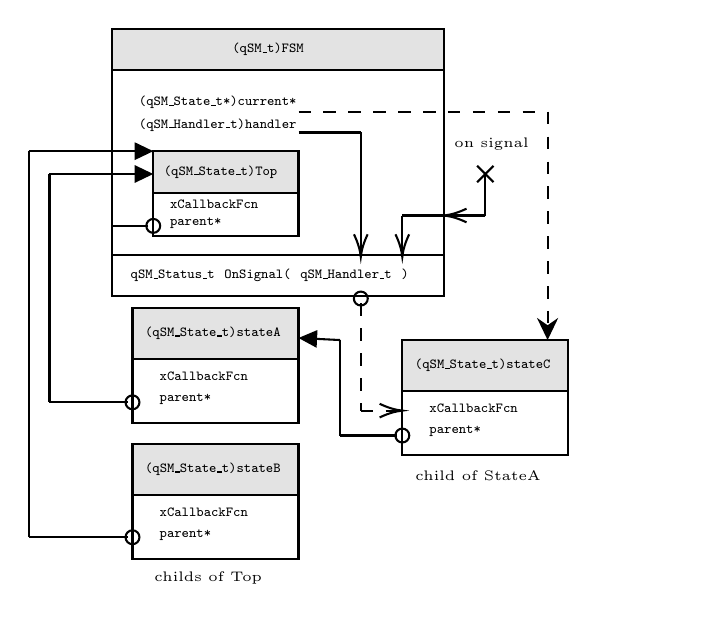
\begin{tikzpicture}[x=0.75pt,y=0.75pt,yscale=-1,xscale=1]
        \draw   (100,40) -- (260,40) -- (260,149) -- (100,149) -- cycle ;
        \draw  [fill={rgb, 255:red, 210; green, 210; blue, 210 }  ,fill opacity=0.62 ] (100,20) -- (260,20) -- (260,40) -- (100,40) -- cycle ;
        \draw   (120,99) -- (190,99) -- (190,120) -- (120,120) -- cycle ;
        \draw  [fill={rgb, 255:red, 210; green, 210; blue, 210 }  ,fill opacity=0.62 ] (120,79) -- (190,79) -- (190,99) -- (120,99) -- cycle ;
        \draw    (60,79) -- (117,79) ;
        \draw [shift={(120,79)}, rotate = 180] [fill=black  ][line width=0.08]  [draw opacity=0] (8.93,-4.29) -- (0,0) -- (8.93,4.29) -- cycle;
        \draw    (60,79) -- (60,265) ;
        \draw   (110,179) -- (190,179) -- (190,210) -- (110,210) -- cycle ;
        \draw  [fill={rgb, 255:red, 210; green, 210; blue, 210 }  ,fill opacity=0.62 ] (110,154.5) -- (190,154.5) -- (190,179) -- (110,179) -- cycle ;
        \draw    (107.65,200) -- (70,200) ;
        \draw [shift={(110,200)}, rotate = 180] [color=black  ][line width=0.75]      (0, 0) circle [x radius= 3.35, y radius= 3.35];
        \draw   (100,129) -- (260,129) -- (260,149) -- (100,149) -- cycle ;
        \draw    (210,170) -- (193,169.15) ;
        \draw [shift={(190,169)}, rotate = 362.86] [fill=black  ][line width=0.08]  [draw opacity=0] (8.93,-4.29) -- (0,0) -- (8.93,4.29) -- cycle    ;
        \draw    (237.65,216) -- (210,216) ;
        \draw [shift={(240,216)}, rotate = 180] [color=black  ][line width=0.75]      (0, 0) circle [x radius= 3.35, y radius= 3.35]   ;
        \draw    (70,90) -- (70,200) ;
        \draw    (70,90) -- (117,90) ;
        \draw [shift={(120,90)}, rotate = 180] [fill=black  ][line width=0.08]  [draw opacity=0] (8.93,-4.29) -- (0,0) -- (8.93,4.29) -- cycle    ;
        \draw    (280,90) -- (280,110) ;
        \draw [shift={(280,90)}, rotate = 135] [color=black  ][line width=0.75]    (-5.59,0) -- (5.59,0)(0,5.59) -- (0,-5.59)   ;
        \draw  [dash pattern={on 4.5pt off 4.5pt}]  (190,60) -- (310,60) ;
        \draw  [dash pattern={on 4.5pt off 4.5pt}]  (310,60) -- (310,167) ;
        \draw [shift={(310,170)}, rotate = 270] [fill=black  ][line width=0.08]  [draw opacity=0] (10.72,-5.15) -- (0,0) -- (10.72,5.15) -- (7.12,0) -- cycle;
        \draw    (280,110) -- (262,110) ;
        \draw [shift={(260,110)}, rotate = 360] [color=black  ][line width=0.75]    (10.93,-3.29) .. controls (6.95,-1.4) and (3.31,-0.3) .. (0,0) .. controls (3.31,0.3) and (6.95,1.4) .. (10.93,3.29)   ;
        \draw    (117.65,115) -- (108.5,115) -- (100,115) ;
        \draw [shift={(120,115)}, rotate = 180] [color=black  ][line width=0.75]      (0, 0) circle [x radius= 3.35, y radius= 3.35]   ;
        \draw    (220,70) -- (220,128) ;
        \draw [shift={(220,130)}, rotate = 270] [color=black  ][line width=0.75]    (10.93,-3.29) .. controls (6.95,-1.4) and (3.31,-0.3) .. (0,0) .. controls (3.31,0.3) and (6.95,1.4) .. (10.93,3.29)   ;
        \draw    (190,70) -- (220,70) ;
        \draw    (210,170) -- (210,216) ;
        \draw  [dash pattern={on 4.5pt off 4.5pt}]  (220,152.35) -- (220,204) ;
        \draw [shift={(220,150)}, rotate = 90] [color=black  ][line width=0.75]      (0, 0) circle [x radius= 3.35, y radius= 3.35]   ;
        \draw  [dash pattern={on 4.5pt off 4.5pt}]  (220,204) -- (238,204) ;
        \draw [shift={(240,204)}, rotate = 180] [color=black  ][line width=0.75]    (10.93,-3.29) .. controls (6.95,-1.4) and (3.31,-0.3) .. (0,0) .. controls (3.31,0.3) and (6.95,1.4) .. (10.93,3.29)   ;
        \draw    (240,110) -- (260,110) ;
        \draw    (240,110) -- (240,128) ;
        \draw [shift={(240,130)}, rotate = 270] [color=black  ][line width=0.75]    (10.93,-3.29) .. controls (6.95,-1.4) and (3.31,-0.3) .. (0,0) .. controls (3.31,0.3) and (6.95,1.4) .. (10.93,3.29)   ;
        \draw    (107.65,265) -- (60,265) ;
        \draw [shift={(110,265)}, rotate = 180] [color=black  ][line width=0.75]      (0, 0) circle [x radius= 3.35, y radius= 3.35]   ;
        \draw   (110,244.5) -- (190,244.5) -- (190,275.5) -- (110,275.5) -- cycle ;
        \draw  [fill={rgb, 255:red, 210; green, 210; blue, 210 }  ,fill opacity=0.62 ] (110,220) -- (190,220) -- (190,244.5) -- (110,244.5) -- cycle ;
        \draw   (240,194.5) -- (320,194.5) -- (320,225.5) -- (240,225.5) -- cycle ;
        \draw  [fill={rgb, 255:red, 210; green, 210; blue, 210 }  ,fill opacity=0.62 ] (240,170) -- (320,170) -- (320,194.5) -- (240,194.5) -- cycle ;
    
        \draw (215,30) node  [font=\ttfamily, text width=3cm] [align=left] {\tiny (qSM\_t)FSM};
        \draw (170,55.5) node  [font=\ttfamily, text width=3cm] [align=left] {\tiny (qSM\_State\_t*)current*};
        \draw (182,89) node  [font=\ttfamily, text width=3cm] [align=left] {\tiny (qSM\_State\_t)Top };
        \draw (185,113.5) node  [font=\ttfamily, text width=3cm] [align=left] {\tiny parent*};
        \draw (173,166.75) node  [font=\ttfamily, text width=3cm] [align=left] {\tiny (qSM\_State\_t)stateA};
        \draw (185,139) node  [font=\ttfamily, text width=4cm] [align=left] {\tiny qSM\_Status\_t OnSignal( qSM\_Handler\_t )};
        \draw (276.5,235.5) node  [font=\tiny] [align=left] {child of StateA};
        \draw (185,104.5) node  [font=\ttfamily, text width=3cm] [align=left] {\tiny xCallbackFcn};
        \draw (180,198.5) node [font=\ttfamily, text width=3cm] [align=left] {\tiny parent*};
        \draw (180,187.5) node  [font=\ttfamily, text width=3cm] [align=left] {\tiny xCallbackFcn};
        \draw (170,66.5) node  [font=\ttfamily, text width=3cm] [align=left] {\tiny (qSM\_Handler\_t)handler};
        \draw (283,75.5) node  [font=\tiny] [align=left] {on signal};
        \draw (173,232.25) node  [font=\ttfamily, text width=3cm] [align=left] {\tiny (qSM\_State\_t)stateB};
        \draw (180,264) node   [font=\ttfamily, text width=3cm] [align=left] {\tiny parent*};
        \draw (180,253) node  [font=\ttfamily, text width=3cm] [align=left] {\tiny xCallbackFcn};
        \draw (146.5,284.5) node  [font=\tiny] [align=left] {childs of Top};
        \draw (303,182.25) node  [font=\ttfamily, text width=3cm] [align=left] {\tiny (qSM\_State\_t)stateC};
        \draw (310,214) node  [font=\ttfamily, text width=3cm] [align=left] {\tiny parent*};
        \draw (310,203) node  [font=\ttfamily, text width=3cm] [align=left] {\tiny xCallbackFcn};
    \end{tikzpicture}
    \caption{FSM module design}
    \label{fig:fsmdesign}
\end{figure}

One important attribute of the \lstinline{qSM_State_t} object is the callback function, which is used to describe the behavior specific to the state. Also there is a pointer to the parent state to define nesting of the state and its place in the hierarchical topology.
As shown in figure \ref{fig:fsmdesign}, a state machine consist of a least one state the "top level" state.
So concrete state machine are built by adding an arbitrary number states and defining callback functions. The only
purpose of the top state is to provide the root of the hierarchy, so that the highest level can return to top as their parent state. 

\subsubsection{Setting up a state machine : \texorpdfstring{\lstinline{qStateMachine_Setup}}{qStateMachine_Setup} }
Like any other OS object, a Finite State Machine (FSM) must be explicitly initialized before it can be used. The \lstinline{qStateMachine_Setup()} API \index{\lstinline{qStateMachine_Setup}}  initializes the instance, sets the callback for the top state, sets the initial state and the surrounding callback function.
\medskip

\begin{lstlisting}[style=CStyle]
qBool_t qStateMachine_Setup(qSM_t * const m, qSM_StateCallback_t topCallback, 
                            qSM_State_t * const initState, 
                            qSM_SurroundingCallback_t surrounding, void *Data )
\end{lstlisting}

\subsubsection*{Parameters}
\begin{itemize}
    \item \lstinline{m} : A pointer to the FSM object.
    \item \lstinline{topCallback} :  The callback for the "Top" state. This argument is a pointer to a callback function, returning \lstinline{qSM_Status_t} and with a \lstinline{qSM_Handler_t} variable as input argument.
    \item \lstinline{initState} : The first state to be executed (initial-state). 
    \item \lstinline{Surrounding} : The surrounding callback function. To ignore pass \lstinline{NULL}.
    \item \lstinline{Data} : Represents the FSM arguments. To ignore pass \lstinline{NULL}. All arguments must be passed by reference and cast to \lstinline{(void *)}. Only one argument is allowed, so, for multiple arguments, create a structure that contains all of the arguments and pass a pointer to that structure. 
\end{itemize}  

\begin{tcolorbox}
\ArrowBoldDownRight \textit{Note}: For the \lstinline{Surrounding} argument, a \lstinline{NULL} value will act as a "disable" action.
\end{tcolorbox}

\subsubsection{Subscribing states and defining callbacks: }
State  machines  are constructed by composition, therefore, the topology of a state machine is determined upon construction.
In this module implementation, there are not distinction between composite states(states containing substates) and leaf states. All states are potentially composite. 
The API \lstinline{qStateMachine_StateSubscribe}\index{\lstinline{qStateMachine_StateSubscribe}} should be used to initialize the state and define its position in the topology.
\medskip

\begin{lstlisting}[style=CStyle]
qBool_t qStateMachine_StateSubscribe( qSM_t * const m, 
                                      qSM_State_t * const state, 
                                      qSM_State_t * const parent, 
                                      qSM_StateCallback_t StateFcn, 
                                      qSM_State_t * const initState, 
                                      void *Data )
\end{lstlisting}

\subsubsection*{Parameters}
\begin{itemize}
    \item \lstinline{m} : a pointer to the FSM object.
    \item \lstinline{state} :  A pointer to the state object.
    \item \lstinline{parent} : A pointer to the parent state. Pass \lstinline{NULL} if this state its a child of the \textit{Top} state.
    \item \lstinline{StateFcn} : The handler function associated to the state. 

                                 Prototype: \lstinline{ qSM_Status_t xCallback( qSM_Handler_t h ) }
    \item \lstinline{initState} : The first child-state to be executed if the subscribed state its a parent in an hierarchical pattern. To ignore pass \lstinline{NULL} as argument.
    \item \lstinline{Data} : State data. Storage pointer. To ignore pass \lstinline{NULL} as argument.
\end{itemize}  

A state callback-functions takes a \lstinline{qSM_Handler_t} object as input argument and returns a \lstinline{qSM_Status_t} value. An example is shown in the following code snippet:
\medskip

\begin{lstlisting}[style=CStyle]
qSM_Status_t ExampleState_Callback( qSM_Handler_t h ){
    /* TODO: State code */
    return qSM_STATUS_EXIT_SUCCESS;
}
\end{lstlisting} 


\subsubsection{The state callback handler : Performing transitions and retrieving data : }

Because callback functions are methods derived from the state-machine object, they have direct access to some attributes via the \lstinline{qSM_Handler_t} argument. 
The usage of this object it's required to make the FSM moves between states and additionally get extra data. The provided attributes are:

\begin{itemize}
    \item \lstinline{NextState} : Desired next state. The application writer should change this field to another state to produce a state transition in the next FSM's cycle. Changing this field will only take effect when the states is executed under user custom-defined signals or in the absence of signals \lstinline{QSM_SIGNAL_NONE}.
    \item \lstinline{StartState} :  Desired nested initial state (substate). The application writer should change this field to set the initial transition if the current state its a parent(or composite state). Changing this field attribute only take effect when the state is executed under the \lstinline{QSM_SIGNAL_START} signal.
    \item \lstinline{Signal} (read-only): Received signal. Can have any of the following values: 
    \begin{itemize}
        \item \lstinline{QSM_SIGNAL_NONE} if no signal available.
        \item \lstinline{QSM_SIGNAL_ENTRY} if the current state has just entered from another state.
        \item \lstinline{QSM_SIGNAL_START} to set nested initial transitions by using the \lstinline{StartState} attribute.
        \item \lstinline{QSM_SIGNAL_EXIT} if the current state has just exit to another state.
        \item Any other user-defined signal will reside here, including the \lstinline{QSM_SIGNAL_TIMEOUT(#)} signals.
    \end{itemize}    
    \item \lstinline{TransitionHistory} : Use this option if the transition is to a composite state. This attribute defines how the story should be handled. If this field is not established, \lstinline{qSM_TRANSITION_NO_HISTORY} is assumed. The possible values for this attribute are:
    \begin{itemize}
        \item \lstinline{qSM_TRANSITION_NO_HISTORY} : History is not preserved. Composite states will start according to their default transition.
        \item \lstinline{qSM_TRANSITION_SHALLOW_HISTORY} : History will be kept to allow the return to only the top-most sub-state of the most recent state configuration, which is entered using the default entry rule.
        \item \lstinline{qSM_TRANSITION_DEEP_HISTORY} : History will be kept to allow full state configuration of the most recent visit to the containing region.
    \end{itemize}
    \item \lstinline{Status} (read-only): The exit(or return) status of the last state. Should be used in the \textit{Surrounding} callback to perform the corresponding actions for every value. On states callback will take the value \lstinline{qSM_STATUS_NULL};
    \item \lstinline{machine} (read-only):  A generic pointer to the container state machine.
    \item \lstinline{Data} (read-only): State-machine associated data. If the FSM is running as a task, the associated event data can be queried through this field. (here, a cast to \lstinline{qEvent_t} is mandatory).
    \item \lstinline{StateData} (read-only): State associated data. Storage-pointer.
\end{itemize}


Within the callback function of every state, only one level of dispatching (based on the signal) is necessary. Typically this is archived using a single-level switch statement.
Callback functions communicate with the state machine engine through the \lstinline{qSM_Handler_t}\index{\lstinline{qSM_Handler_t}} and the return value of type \lstinline{qSM_Status_t}.

The semantic is simple, if a signal is processed, the callback functions returns the status value \lstinline{qSM_STATUS_SIGNAL_HANDLED}. otherwise it throws the signal for further processing by higher-level states. Also, this returning mechanism can be used to handle exceptions by using the surrounding callback.

\textit{Entry/Exit} actions and default transitions are also implemented inside the callback function in response of pre-defined signals. \lstinline{QSM_SIGNAL_ENTRY}, \lstinline{QSM_SIGNAL_EXIT} and \lstinline{QM_SIGNAL_START}.
The state machine generates and dispatches this signals to appropriates handlers upon state transitions.

The example below shows what a status callback should look like including the use of the handler.
\medskip

\begin{lstlisting}[style=CStyle]
qSM_Status_t ExampleState_Callback( qSM_Handler_t h ){
    switch( h ){
        case QSM_SIGNAL_START:
            break;
        case QSM_SIGNAL_ENTRY:
            break;
        case QSM_SIGNAL_EXIT:
            break;
        case USER_DEFINED_SIGNAL:
            h->NextState  =  &OtherState; /*transition*/
            break;
        default:
            break;
    }
    return qSM_STATUS_EXIT_SUCCESS;
}
\end{lstlisting} 

As shown above, the return value represents the exit status of the state, and it can be handled with an additional \textit{surrounding} callback function ($S_u$) established at the moment of the FSM setup. The values allowed to return are listed below.

\begin{itemize}
    \item \lstinline{qSM_STATUS_EXIT_SUCCESS}.
    \item \lstinline{qSM_STATUS_EXIT_FAILURE}.
    \item \lstinline{qSM_STATUS_SIGNAL_HANDLED}.
    \item Any other integer value between \lstinline{-32762} and \lstinline{32767}.
\end{itemize} 


To code initial transitions, application writer should catch the \lstinline{QSM_SIGNAL_START}, perform the required actions and then designate the target sub-state by assigning the \lstinline{StartState} attribute of the \lstinline{qSM_Handler_t} argument.
Regular transitions are coded in a very similar way, except that here, you catch the custom-defined signal and then assign the \lstinline{NextState} attribute of the \lstinline{qSM_Handler_t} argument.
The developer is free to write and control state transitions. Transitions are only allowed under the availability of user custom-defined signals. Regular transitions are not allowed at an entry point (\lstinline{QSM_SIGNAL_ENTRY}), exit point (\lstinline{QSM_SIGNAL_EXIT}), or a start point (\lstinline{QSM_SIGNAL_START}).

\begin{tcolorbox}
\ArrowBoldDownRight \textit{Note}: User should not target the top state in a transition and use it as transition source either. The only customizable aspect of the top state is the initial transition.
\end{tcolorbox}

\subsubsection{The surrounding callback}
It is a checkpoint before and after each state executes its activities through its state-callback. The behavior of this surrounding callback must be defined by the programmer.

\begin{figure}[H]
    \centering
    \begin{tikzpicture}[initial text={...}, ->,>=stealth',shorten >=1pt,auto,node distance=1.8cm, semithick]
        \draw[dotted] (0.8,-1) -- (6.2,-1) -- (6.2,1) -- (0.8,1) -- (0.8,-1 ) -- cycle;
        \node[dashed, initial,state]            (A)              {$P_{-1}$};
        \node[fill=gray!20, state]              (B) [right of=A] {$S_u$};
        \node[fill=gray!80, state, accepting]   (C) [right of=B] {$P$};
        \node[fill=gray!20, state]              (D) [right of=C] {$S_u$};
        \node[dashed, state]                    (E) [right of=D] {$P_{+1}$};
        \node[state,draw=none]                  (H) [right of=E] {};
        %\node at (9.99, 0.4)   (D1) [font=\ttfamily, text width=2cm]{\tiny NextState};    
        %\node at (9.99, 0.2)   (D2) [font=\ttfamily, text width=2cm]{\tiny = P+1};  
        %\node at (9.99, 2.2)   (D3) [font=\ttfamily, text width=2cm]{\tiny NextState};
        %\node at (9.99, 2.0)   (D4) [font=\ttfamily, text width=2cm]{\tiny unchanged};
        %\node at (6.40, 1.2)   (D4) [font=\ttfamily, text width=2cm, rotate=45]{\tiny qSM\_EXIT\_SUCCESS};
        %\node at (6.4, -1.2)   (D4) [font=\ttfamily, text width=2cm, rotate=-45]{\tiny qSM\_EXIT\_FAILURE};
        %\node at (6.99, 0.2)   (D4) [font=\ttfamily, text width=2cm]{\tiny -32766};
        %\node at (6.89, -0.2)   (D4) [font=\ttfamily, text width=2cm]{\tiny to 32767};
        \node at (0.3,-0.8)   (D5) [text width=1.5cm]{\tiny Previous};    
        \node at (2.1,-0.8)   (D6) [text width=1.5cm]{\tiny BeforeAny};
        \node at (4.0,-0.8)   (DX) [text width=1.5cm]{\tiny Current};
        %\node at (3.9,-0.4)   (DY) [text width=1.5cm]{\tiny table};
        %\node at (3.9,-0.6)   (DY) [text width=1.5cm]{\tiny evaluation};
        \node at (5.65,-0.8)   (D7) [text width=1.5cm]{\tiny $P$ return value};
        \node at (7.6,-0.8)    (D8) [text width=1.5cm]{\tiny Next};
        %\node at (7.29,-0.6)   (D9) [text width=1.5cm]{\tiny Unexpected};
        %\node at (7.59,-2.5)   (DA) [text width=1.5cm]{\tiny Failure};
        %\node at (11.29,-0.8)   (DB) [text width=1.5cm]{\tiny Other};

        \path   (A) edge node {} (B)
                (B) edge node {} (C) 
                (C) edge node {} (D)
                (D) edge node {} (E);
                (E) edge node {} (H);
    \end{tikzpicture}
    \caption{Surrounding callback ($S_u$) invocation after and before the \textit{current} state ($P$)}
    \label{fig:substates}
\end{figure}

When the surrounding callback is executed, it indicates its own checkpoint through the \lstinline{Status} attribute of the \lstinline{qSM_Handler_t} argument.

Unlike a state callback, the \textit{Surrounding} callback should not return anything, thus, the callback should be written as:
\medskip

\begin{lstlisting}[style=CStyle]
void SurroundingCallback_Example( qSM_Handler_t m ){
    switch( h->Status ){
        case qSM_STATUS_BEFORE_ANY:
            /* TODO: before any code */
            break;
        case qSM_STATUS_EXIT_FAILURE:
            /* TODO: failure code */
            break;
        case qSM_STATUS_EXIT_SUCCESS:
            /* TODO: success code */
            break;
        case qSM_STATUS_SIGNAL_HANDLED:
            /* TODO: signal handled code */
            break;            
        case 5: /*user defined return value*/ 
            /* TODO: used defined*/
            break;
        default: 
            /*handle the unexpected*/
            break
    }
}
\end{lstlisting}  

As you can see in the example below, the surrounding execution case its checked through the FSM handle by reading the \lstinline{Status} field.

\subsubsection{Running a state machine : \texorpdfstring{\lstinline{qStateMachine_Run}}{qStateMachine_Run} }

This API \index{\lstinline{qStateMachine_Run}} is used to execute the Finite State Machine. Only a single cycle is performed propagating the input signal until it is handled.
\medskip

\begin{lstlisting}[style=CStyle]
qBool_t qStateMachine_Run( qSM_t * const m, qSM_Signal_t xSignal )
\end{lstlisting}

\subsubsection*{Parameters}
\begin{itemize}
    \item \lstinline{obj} : a pointer to the FSM object.
    \item \lstinline{xSignal} :  User-defined signal (this value will be ignored if the installed queue has items available)
\end{itemize}  

\subsubsection{Adding a state machine as a task : \texorpdfstring{\lstinline{qOS_Add_StateMachineTask}}{qOS_Add_StateMachineTask} } \label{statemachinetask}
The best strategy to run a FSM is delegating it to a task. For this, the provided \index{\lstinline{qOS_Add_StateMachineTask}} API should be used. Here, the task doesn't have a specific callback, instead, it will evaluate the active state of the FSM, and later, all the other possible states in response to events that mark their own transition. The task will be scheduled to run every \lstinline{Time} seconds in \lstinline{qPeriodic} mode. 

Using this API, the kernel will take care of the FSM by itself, so the usage of \lstinline{qStateMachine_Run()} can be omitted. 
\medskip

\begin{lstlisting}[style=CStyle]
qBool_t qOS_Add_StateMachineTask( qTask_t * const Task, qSM_t *m, 
                                  qPriority_t Priority, 
                                  qTime_t Time, qState_t InitialTaskState,
                                  void *arg )
\end{lstlisting}

\subsubsection*{Parameters}
\begin{itemize}
    \item \lstinline{Task} : A pointer to the task node. 
    \item \lstinline{m} : A pointer to Finite State-Machine (FSM) object.
    \item \lstinline{Priority} : The priority value. [0(min) - \lstinline{Q_PRIORITY_LEVELS}(max)]
    \item \lstinline{Time} : Execution interval defined in seconds (floating-point format). For immediate execution use the  \lstinline{qTimeImmediate} definition. 
    \item \lstinline{InitialTaskState } : Specifies the initial operational state of the task (\lstinline{qEnabled}, \lstinline{qDisabled}, \lstinline{qAsleep} or \lstinline{qAwake}).
    \item \lstinline{arg} - Represents the task arguments. All arguments must be passed by reference and cast to \lstinline{(void *)}. 
\end{itemize}

\begin{tcolorbox}
\ArrowBoldDownRight \textit{Note}: For the \lstinline{Surrounding} argument, a \lstinline{NULL} value will act as a disable action.
\end{tcolorbox}

Now that a task is running a dedicated state-machine, the specific task event-info can be obtained in every state callback through the \lstinline{Data} field of the \lstinline{qSM_Handler_t} argument. Check the example below:
\medskip

\lstinputlisting[style=CStyle]{sec3fsmtaskinfo.c}

\subsubsection{A demonstrative example} \label{fsm_example}
In this example, one press of the button turn on the LED, a second push of the button will make the LED blink and if the button is pressed again, the LED will turn off. Also, our system must turn off the LED after a period of inactivity. If the button hasn't been pressed in the last 10 seconds, the LED will turn off. 

States ($\ S_i$) and transitions ($\ t_i$) are described as follows: 
\medskip
\begin{itemize}
\begin{minipage}{0.4\linewidth}
    \item $\ S_1$ : LED Off
    \item $\ S_2$ : LED On
    \item $\ S_3$ : LED Blink
\end{minipage}
\begin{minipage}{0.4\linewidth}
    \item $\ t_1$ : Button press (rising edge)
    \item $\ t_2$ : Timeout (10S)
\end{minipage}
\end{itemize}

\begin{figure}[H]
    \centering 
    \begin{tikzpicture}[->,>=stealth',shorten >=1pt,auto,node distance=2.8cm, semithick]
        \node[initial,state] (A)                    {$S_1$};
        \node[state]         (B) [above right of=A] {$S_2$};
        \node[state]         (C) [below right of=B] {$S_3$};
    
        \path   (A) edge [bend left]  node {$t_1$} (B)
                (B) edge              node {$t_1$} (C)
                (C) edge [bend left]  node {$t_1$} (A)
                (C) edge              node {$t_2$} (A)
                (B) edge [bend left]  node {$t_2$} (A);
    \end{tikzpicture}
    \caption{A simple FSM example with three states}
    \label{fig:fsmexample}
\end{figure}

To start the implementation, let's define the necessary global variables...

\begin{lstlisting}[style=CStyle]
qTask_t LED_Task; /*The task node*/
qSM_t LED_FSM; /*The state-machine handle*/
qSM_State_t State_LEDOff, State_LEDOn, State_LEDBlink;
\end{lstlisting}

Then, we define our states as the flow-diagram showed in figure \ref{fig:fsmexample}.

\lstinputlisting[style=CStyle]{sec3fsmledexample.c}

Finally, we add the task to the scheduling scheme running the dedicated state machine.

Remember that you must set up the scheduler before adding a task to the scheduling scheme.
\medskip

\begin{lstlisting}[style=CStyle]
qStateMachine_Setup( &LED_FSM, NULL, &State_LEDOff, NULL, NULL ); 
qStateMachine_StateSubscribe( &LED_FSM, &State_LEDOff, NULL, 
                              State_LEDOff_Callback, NULL, NULL ); 
qStateMachine_StateSubscribe( &LED_FSM, &State_LEDOn, NULL, 
                              State_LEDOn_Callback, NULL, NULL );
qStateMachine_StateSubscribe( &LED_FSM, &State_LEDBlink, NULL, 
                              State_LEDBlink_Callback, NULL, NULL ); 
qOS_Add_StateMachineTask( &LED_Task, &LED_FSM, qHigh_Priority, 
                          0.1, qEnabled, NULL );
\end{lstlisting}


\subsubsection{Sending signals}
To communicate within and between state-machines or even other contexts, use signals. A signal\index{\lstinline{qSM_Signal_t}} is a simple value who can be used to abstract an incoming event. In the receiving state-machine, a queue or a exclusion variable receives the signal and holds it until the state-machine can evaluate it.

When coding state-machines, the application writer can benefit from this simple event-abstraction mechanism. On the one hand, there would be a more uniform programming when writing states callbacks and on the other hand, the communication of the state machine from other contexts becomes easier.

To send a signal to a state machine, use the following API:
\medskip

\begin{lstlisting}[style=CStyle]
 qBool_t qStateMachine_SendSignal( qSM_t * const m, qSM_Signal_t xSignal, 
                                   const qBool_t isUrgent )
\end{lstlisting} \index{\lstinline{qStateMachine_SendSignal}}

\subsubsection*{Parameters}
\begin{itemize}
    \item \lstinline{m} : A pointer to the FSM object. 
    \item \lstinline{xSignal} : The user-defined signal.
    \item \lstinline{isUrgent} : If \lstinline{qTrue}, the signal will be sent to the front of the queue. (only if the there is a signal-queue available)
\end{itemize}

\subsubsection*{Return Value}
\lstinline{qTrue} on success, otherwise returns \lstinline{qFalse}.

\lstinline{qFalse} if there is a queue, and the signal cannot be inserted because it is full or the exclusion variable has not been freed.

\hrulefill
\medskip

This API can manage their delivery to one of these possible destinations: an \textit{exclusion variable} or a \textit{signal queue}:
\begin{itemize}
    \item An \textit{exclusion variable} its a variable with an important distinction, it can only be written if it is empty. The empty situation only happens, if the engine has already propagated the signal within the state machine. If the signal has not yet propagated, the signal sending cannot be carried out.
    \item When a \textit{signal queue} is used, the signal is put into a FIFO structure and the engine takes care of dispatching the signal in an orderly manner. The only situation where the signal cannot be delivered is if the queue is full.
    This its the preferred destination, as long as there is a previously installed signal queue (for this, please review the next section.
\end{itemize}

\begin{tcolorbox}
\ArrowBoldDownRight \textit{Note}: If the signal-queue its available, the \lstinline{qStateMachine_SendSignal} will always select it as destination.
\end{tcolorbox}

\begin{tcolorbox}
\ArrowBoldDownRight If a state-machine, a task, or another context sends a signal to a full queue, an queue-overflow occurs. The result of the queue overflow it that the state-machine drops the new signal. 
\end{tcolorbox}

\subsubsection{Installing a signal queue}
A state machine can have a FIFO queue to allow the delivery of signals from another contexts. If the signal queue its installed, the state-machine engine constantly monitors the queue for available signals. The engine then propagates the signal through the hierarchy until it is processed. 
To enable this functionality in your state machine, the queue must be installed by using the \lstinline{qStateMachine_InstallSignalQueue} API.

The install operation should be performed after both, the queue and the FSM are correctly initialized by using \lstinline{qQueue_Setup} and \lstinline{qStateMachine_Setup} respectively.
\medskip

\begin{lstlisting}[style=CStyle]
qBool_t qStateMachine_InstallSignalQueue( qSM_t * const m, qQueue_t *queue );
\end{lstlisting} \index{\lstinline{qStateMachine_InstallSignalQueue}}

\subsubsection*{Parameters}
\begin{itemize}
    \item \lstinline{m} : A pointer to the FSM object. 
    \item \lstinline{queue} : A pointer to the queue instance. 
\end{itemize}

\subsubsection*{Return Value}
\lstinline{qTrue} on success, otherwise returns \lstinline{qFalse}.

\hrulefill
\medskip

\begin{tcolorbox}
\ArrowBoldDownRight \textit{Note}: Make sure that queues are enabled in the \lstinline{qconfig.h}.
\end{tcolorbox}

\begin{tcolorbox}
\HandRight When configuring a signal queue with \lstinline{qQueue_Setup}, remember to size it based on the type \lstinline{qSM_Signal_t}.
\end{tcolorbox}

\begin{tcolorbox}
\HandRight If the state-machines its delegated to a task, make sure to install the queue prior to setting up the task. In this way, a kernel connection can be performed between the FSM signal-queue and the FSM-task, allowing the OS to catch signals to produce a task event, this prevents the wait of the task for the specified period, resulting in a faster handling of incoming signals.
\end{tcolorbox}

\subsubsection{Using a transition table}
In this approach, the FSM is coded in tables with the outgoing transitions of every state, where each entry relates signals, actions and the target state.
This is an elegant method to translate the FSM to actual implementation as the handling for every state and event combination is encapsulated in the table. 

\begin{table}[H]
\centering
\begin{tabular}{||c c c c||} 
 \hline
  \textit{Signal} & \textit{Signal action/guard} & \textit{Target state}& \textit{History mode}  \\ [0.5ex] 
 
 \hline\hline
 \ttfamily{Signal1} & \ttfamily{NULL} & \ttfamily{StateB} & 0 \\ 
 \ttfamily{Signal3} & \ttfamily{DoOnSignal3} & \ttfamily{StateD} & 0 \\
 ... & ... & ... & ... \\
 \ttfamily{Signal6} & \ttfamily{NULL} & \ttfamily{StateA} & 0 \\ [1ex] 
 \hline
\end{tabular}
\caption{Transition table layout for a state}
\label{ttable_layout}
\end{table}

Here, the application writer get a quick picture of the FSM and the embedded software maintenance is also much more under control. A transition should be explicitly installed in the target state with the corresponding entries, an \textit{n}-sized array of \lstinline{qSM_Transition_t}\index{\lstinline{qSM_Transition_t}} elements. 

The API \lstinline{qStateMachine_InstallTransitionTable()}, should be used to perform the transition table installation to a specific state.
\medskip

\begin{lstlisting}[style=CStyle]
qBool_t qStateMachine_Set_StateTransitions( qSM_State_t * const state,
                                            qSM_Transition_t * const table,
                                            const size_t n )
\end{lstlisting} \index{\lstinline{qStateMachine_Set_StateTransitions}}

\subsubsection*{Parameters}
\begin{itemize}
    \item \lstinline{m} : A pointer to the state object. 
    \item \lstinline{table} : The array of entries (\lstinline{qSM_Transition_t[]}) that describes the outgoing transitions. 
    \item \lstinline{n} : The number of transitions available within the \lstinline{table}.
\end{itemize}

\subsubsection*{Return Value}
Returns \lstinline{qTrue} on success, otherwise returns \lstinline{qFalse}.

\hrulefill

\subsubsection*{Caveats}
\begin{itemize}
    \item State transitions are not limited to the specification of the transition table. A state callback owns the higher precedence to change a state. The application writer can use both, a transition table and direct \lstinline{NextState} field manipulation in state callbacks to perform a transition to the FSM.
    \item Special care is required when the table grows very large, that is, when there are many invalid state/event combinations, leading to a waste of memory. There is also a memory penalty as the number of states and events grow. The application writer  need to accurately account for this during initial design. A statechart pattern can be used to improve the design and reduce the number of transition entries. 
    \item The user is responsible for defining the transitions according to the topology of the state machine. Undefined behaviors can occur if the topology is broken with poorly defined transitions.
\end{itemize}


\begin{tcolorbox}
\ArrowBoldDownRight \textit{Note}: When a transition entry is defined. the event-signal should be located as the second parameter of the entry. Please see the transition layout in table \ref{ttable_layout}.
\end{tcolorbox}

\subsubsection{Signal actions and guards:} 
Transition tables allow the usage of this feature. When an event-signal is received from the queue, the signal-action, if available, is evaluated before the transition is triggered. This action is user-defined and should be coded as a function that takes a \lstinline{qSM_Handler_t} object and returns a value of type \lstinline{qBool_t}. 
\medskip

\begin{lstlisting}[style=CStyle]
qBool_t Signal_Action( qSM_Handler_t h ){
    /* TODO : Event-signal action*/
    return qTrue; /*allow the state transition*/
}
\end{lstlisting}

The return value is checked after to allow or reject the state transition. The application writer can code a boolean expression to implement statechart guards or perform some pre-transition procedure.

\begin{tcolorbox}
\HandRight If a signal-action returns \lstinline{qFalse}, the event-signal is rejected, preventing the state transition to be performed in the calling FSM.
\end{tcolorbox}

\begin{tcolorbox}
\ArrowBoldDownRight \textit{Note}: When a transition entry is defined. the signal-action should be located as the third parameter of the entry. Please see the transition layout in table \ref{ttable_layout}.
A \lstinline{NULL} value will act as a NOT-defined, always allowing the state-transition. 
\end{tcolorbox}


\subsubsection{FSM Timeout specification}
A timeout specification is mechanism to simplify the notion of time passage inside states. The basic usage model of the timeout signals is as follows:

An timeout specification allocates one or more timer objects. The user relates in a table each specific timeout operations within the state where are they going to operate. So, according to the table, when a state needs to arrange for a timeout, the engine can set or reset the given timer.  When the FSM engine detects that the appropriate moment has arrived (a timer expiration occurs), it inserts the timeout signal directly into the recipient's event queue. The recipient then processes the timeout signal just like any other signal.

Given the above explanation, it is evident that for its operation, the state machine requires an installed signal queue.

A timeout specification is referenced by an object of type \lstinline{qSM_TimeoutSpec_t}\index{\lstinline{qSM_TimeoutSpec_t}} and must be installed inside the state machine using the API \lstinline{qStateMachine_InstallTimeoutSpec()}.
\medskip

\begin{lstlisting}[style=CStyle]
qBool_t qStateMachine_InstallTimeoutSpec( qSM_t * const m,  
                                          qSM_TimeoutSpec_t * const ts );
\end{lstlisting} \index{\lstinline{qStateMachine_InstallTimeoutSpec}}

\subsubsection*{Parameters}
\begin{itemize}
    \item \lstinline{m} : A pointer to the FSM object. 
    \item \lstinline{ts} : A pointer to the timeout specification object.
\end{itemize}

\subsubsection*{Return Value}
Returns \lstinline{qTrue} on success, otherwise returns \lstinline{qFalse}.

\hrulefill

Then, timeout operations can be defined in a table for each state using the following  API:

\begin{lstlisting}[style=CStyle]
qBool_t qStateMachine_Set_StateTimeouts( qSM_State_t * const state, 
                                         qSM_TimeoutStateDefinition_t *tdef, 
                                         const size_t n  );
\end{lstlisting} \index{\lstinline{qStateMachine_Set_StateTimeouts}}

\subsubsection*{Parameters}
\begin{itemize}
    \item \lstinline{state} : A pointer to the state object. 
    \item \lstinline{tdef} : The lookup table matching the requested timeout values with their respective options.
    \item \lstinline{n} : the number of elements inside \lstinline{tdef}.
\end{itemize}

\subsubsection*{Return Value}
Returns \lstinline{qTrue} on success, otherwise returns \lstinline{qFalse}.

A timeout specification element  is defined as an structure of type \lstinline{qSM_TimeoutStateDefinition_t}\index{\lstinline{qSM_TimeoutStateDefinition_t}} and should follow this layout:

\begin{table}[H]
\centering
\begin{tabular}{||c c||} 
 \hline
 \textit{Timeout value} & \textit{Options} \\ [0.5ex] 
 \hline
\end{tabular}
\caption{Timeout specification layout}
\label{timeoutspec_table_layout}
\end{table}

The options for every timeout its a bitwise value that indicates which timeout should be used and the operations than should be performed internally by the state-machine engine. This options can be combined with a bitwise OR and are detailed as follows:

\begin{itemize}
    \item \lstinline{QSM_TSOPT_INDEX(index)} : To select the timeout to be used in the specification. Should be a value between \lstinline{0} and \lstinline{(Q_FSM_MAX_TIMEOUTS-1)}
    \item \lstinline{QSM_TSOPT_SET_ENTRY} : To set the timeout when the specified state its entering.
    \item \lstinline{QSM_TSOPT_RST_ENTRY} :  To reset the timeout when the specified state its entering.
    \item \lstinline{QSM_TSOPT_SET_EXIT} : To set the timeout when the specified state its exiting.
    \item \lstinline{QSM_TSOPT_RST_EXIT} : To reset the timeout when the specified state its exiting.
    \item \lstinline{QSM_TSOPT_KEEP_IF_SET} : To apply the Set operation only if the timeout its in a reset state.
    \item \lstinline{QSM_TSOPT_PERIODIC} : To put the timeout in periodic mode.
\end{itemize}

\begin{tcolorbox}
\HandRight The user is responsible for writing timeout specifications correctly. Care must be taken that the specifications do not collide between hierarchical states to avoid overwriting operations.
\end{tcolorbox}

\begin{tcolorbox}
\HandRight You can increase the number of available timeouts instances by changing the \lstinline{Q_FSM_MAX_TIMEOUTS} configuration macro inside \lstinline{qconfig.h}. 
\end{tcolorbox}

\subsubsection{Demonstrative example using transition tables}
The following example shows the implementation of the FSM presented in section \ref{fsm_example} using the transition table approach with signal-queue and a timeout specification.

Before getting started, the required variables should be defined: 
\medskip

\lstinputlisting[style=CStyle]{sec3fsmledttabledef.c}

Then, we define the callback for the states.
\medskip

\lstinputlisting[style=CStyle]{sec3fsmledttablestates.c}

In the previous code snippet, we assumed that \lstinline{SIGNAL_BUTTON_PRESSED} can be delivered from either the interrupt context or another task.

To finish the setup, a task is added to handle the FSM and then, the transition table can be installed with the other required objects.
\medskip

\lstinputlisting[style=CStyle]{sec3fsmledttablesetup.c}

\subsubsection{Demonstrative example using the hierarchical approach} 
In conventional state machine designs, all states are considered at the same level. The design does not capture the commonality that exists among states. In real life, many states handle most transitions in similar fashion and differ only in a few key components. Even when the actual handling differs, there is still some commonality. It is in these situations where the hierarchical designs makes the most sense.

\begin{figure}[H]
    \centering



\tikzset{every picture/.style={line width=0.75pt}} %set default line width to 0.75pt        

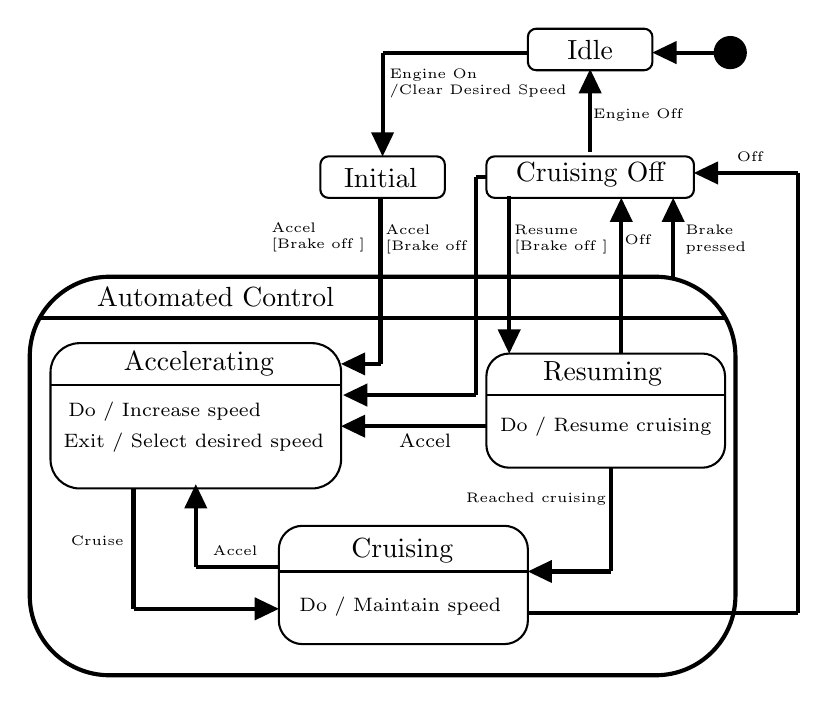
\begin{tikzpicture}[x=0.75pt,y=0.75pt,yscale=-1,xscale=1]
%uncomment if require: \path (0,423); %set diagram left start at 0, and has height of 423

%Rounded Rect [id:dp6662432613291265] 
\draw   (350,77.5) .. controls (350,75.29) and (351.79,73.5) .. (354,73.5) -- (406,73.5) .. controls (408.21,73.5) and (410,75.29) .. (410,77.5) -- (410,89.5) .. controls (410,91.71) and (408.21,93.5) .. (406,93.5) -- (354,93.5) .. controls (351.79,93.5) and (350,91.71) .. (350,89.5) -- cycle ;
%Rounded Rect [id:dp6675663074581135] 
\draw   (330,139) .. controls (330,136.79) and (331.79,135) .. (334,135) -- (426,135) .. controls (428.21,135) and (430,136.79) .. (430,139) -- (430,151) .. controls (430,153.21) and (428.21,155) .. (426,155) -- (334,155) .. controls (331.79,155) and (330,153.21) .. (330,151) -- cycle ;
%Rounded Rect [id:dp4902980476857408] 
\draw   (250,139) .. controls (250,136.79) and (251.79,135) .. (254,135) -- (306,135) .. controls (308.21,135) and (310,136.79) .. (310,139) -- (310,151) .. controls (310,153.21) and (308.21,155) .. (306,155) -- (254,155) .. controls (251.79,155) and (250,153.21) .. (250,151) -- cycle ;
%Rounded Rect [id:dp04982037628337932] 
\draw  [line width=1.5]  (110,231.4) .. controls (110,210.19) and (127.19,193) .. (148.4,193) -- (411.6,193) .. controls (432.81,193) and (450,210.19) .. (450,231.4) -- (450,346.6) .. controls (450,367.81) and (432.81,385) .. (411.6,385) -- (148.4,385) .. controls (127.19,385) and (110,367.81) .. (110,346.6) -- cycle ;
%Straight Lines [id:da7764377667791469] 
\draw [line width=1.5]    (115,213) -- (445,213) ;
%Rounded Rect [id:dp3592571098130719] 
\draw   (120,239) .. controls (120,231.27) and (126.27,225) .. (134,225) -- (246,225) .. controls (253.73,225) and (260,231.27) .. (260,239) -- (260,281) .. controls (260,288.73) and (253.73,295) .. (246,295) -- (134,295) .. controls (126.27,295) and (120,288.73) .. (120,281) -- cycle ;
%Straight Lines [id:da12221010491803885] 
\draw    (120,245) -- (260,245) ;
%Straight Lines [id:da7923623652305394] 
\draw [line width=1.5]    (380,133) -- (380,97) ;
\draw [shift={(380,93)}, rotate = 450] [fill={rgb, 255:red, 0; green, 0; blue, 0 }  ][line width=0.08]  [draw opacity=0] (11.61,-5.58) -- (0,0) -- (11.61,5.58) -- cycle    ;
%Straight Lines [id:da4788139730465273] 
\draw [line width=1.5]    (280,85) -- (280,131) ;
\draw [shift={(280,135)}, rotate = 270] [fill={rgb, 255:red, 0; green, 0; blue, 0 }  ][line width=0.08]  [draw opacity=0] (11.61,-5.58) -- (0,0) -- (11.61,5.58) -- cycle    ;
%Straight Lines [id:da6292308218465252] 
\draw [line width=1.5]    (280,85) -- (350,85) ;
%Straight Lines [id:da0875450823970263] 
\draw [line width=1.5]    (279,155) -- (279,235) ;
%Straight Lines [id:da699195185218056] 
\draw [line width=1.5]    (279,235) -- (264,235) ;
\draw [shift={(260,235)}, rotate = 360] [fill={rgb, 255:red, 0; green, 0; blue, 0 }  ][line width=0.08]  [draw opacity=0] (11.61,-5.58) -- (0,0) -- (11.61,5.58) -- cycle    ;
%Rounded Rect [id:dp8856700522665595] 
\draw   (330,241) .. controls (330,234.92) and (334.92,230) .. (341,230) -- (434,230) .. controls (440.08,230) and (445,234.92) .. (445,241) -- (445,274) .. controls (445,280.08) and (440.08,285) .. (434,285) -- (341,285) .. controls (334.92,285) and (330,280.08) .. (330,274) -- cycle ;
%Straight Lines [id:da9945138562971891] 
\draw    (330,250) -- (445,250) ;
%Straight Lines [id:da6156951818554592] 
\draw [line width=1.5]    (330,265) -- (264,265) ;
\draw [shift={(260,265)}, rotate = 360] [fill={rgb, 255:red, 0; green, 0; blue, 0 }  ][line width=0.08]  [draw opacity=0] (11.61,-5.58) -- (0,0) -- (11.61,5.58) -- cycle    ;
%Rounded Rect [id:dp5701769675760315] 
\draw   (230,324.4) .. controls (230,318.1) and (235.1,313) .. (241.4,313) -- (338.6,313) .. controls (344.9,313) and (350,318.1) .. (350,324.4) -- (350,358.6) .. controls (350,364.9) and (344.9,370) .. (338.6,370) -- (241.4,370) .. controls (235.1,370) and (230,364.9) .. (230,358.6) -- cycle ;
%Straight Lines [id:da16447218181580947] 
\draw    (230,335) -- (350,335) ;
%Straight Lines [id:da8763315052436695] 
\draw [line width=1.5]    (190,333) -- (190,297) ;
\draw [shift={(190,293)}, rotate = 450] [fill={rgb, 255:red, 0; green, 0; blue, 0 }  ][line width=0.08]  [draw opacity=0] (11.61,-5.58) -- (0,0) -- (11.61,5.58) -- cycle    ;
%Straight Lines [id:da04338392142075098] 
\draw [line width=1.5]    (190,333) -- (230,333) ;
%Straight Lines [id:da5695037590069909] 
\draw [line width=1.5]    (160,353) -- (226,353) ;
\draw [shift={(230,353)}, rotate = 180] [fill={rgb, 255:red, 0; green, 0; blue, 0 }  ][line width=0.08]  [draw opacity=0] (11.61,-5.58) -- (0,0) -- (11.61,5.58) -- cycle    ;
%Straight Lines [id:da10244373323079281] 
\draw [line width=1.5]    (160,295) -- (160,353) ;
%Straight Lines [id:da8658544131618406] 
\draw [line width=1.5]    (390,335) -- (354,335) ;
\draw [shift={(350,335)}, rotate = 360] [fill={rgb, 255:red, 0; green, 0; blue, 0 }  ][line width=0.08]  [draw opacity=0] (11.61,-5.58) -- (0,0) -- (11.61,5.58) -- cycle    ;
%Straight Lines [id:da7034657843967269] 
\draw [line width=1.5]    (390,285) -- (390,335) ;
%Straight Lines [id:da5226411692819652] 
\draw [line width=1.5]    (480,143) -- (434,143) ;
\draw [shift={(430,143)}, rotate = 360] [fill={rgb, 255:red, 0; green, 0; blue, 0 }  ][line width=0.08]  [draw opacity=0] (11.61,-5.58) -- (0,0) -- (11.61,5.58) -- cycle    ;
%Straight Lines [id:da01310825459474807] 
\draw [line width=1.5]    (480,143) -- (480,355) ;
%Straight Lines [id:da8077248116651661] 
\draw [line width=1.5]    (350,355) -- (480,355) ;
%Straight Lines [id:da581938331155091] 
\draw [line width=1.5]    (420,193) -- (420,159) ;
\draw [shift={(420,155)}, rotate = 450] [fill={rgb, 255:red, 0; green, 0; blue, 0 }  ][line width=0.08]  [draw opacity=0] (11.61,-5.58) -- (0,0) -- (11.61,5.58) -- cycle    ;
%Straight Lines [id:da5646686872608353] 
\draw [line width=1.5]    (395,230) -- (395,159) ;
\draw [shift={(395,155)}, rotate = 450] [fill={rgb, 255:red, 0; green, 0; blue, 0 }  ][line width=0.08]  [draw opacity=0] (11.61,-5.58) -- (0,0) -- (11.61,5.58) -- cycle    ;
%Straight Lines [id:da777864348657342] 
\draw [line width=1.5]    (341,154) -- (341,226) ;
\draw [shift={(341,230)}, rotate = 270] [fill={rgb, 255:red, 0; green, 0; blue, 0 }  ][line width=0.08]  [draw opacity=0] (11.61,-5.58) -- (0,0) -- (11.61,5.58) -- cycle    ;
%Shape: Circle [id:dp37606004244595703] 
\draw  [fill={rgb, 255:red, 0; green, 0; blue, 0 }  ,fill opacity=1 ] (440,85) .. controls (440,80.86) and (443.36,77.5) .. (447.5,77.5) .. controls (451.64,77.5) and (455,80.86) .. (455,85) .. controls (455,89.14) and (451.64,92.5) .. (447.5,92.5) .. controls (443.36,92.5) and (440,89.14) .. (440,85) -- cycle ;
%Straight Lines [id:da3457264380323728] 
\draw [line width=1.5]    (440,85) -- (414,85) ;
\draw [shift={(410,85)}, rotate = 360] [fill={rgb, 255:red, 0; green, 0; blue, 0 }  ][line width=0.08]  [draw opacity=0] (11.61,-5.58) -- (0,0) -- (11.61,5.58) -- cycle    ;
%Straight Lines [id:da19616464722638915] 
\draw [line width=1.5]    (325,250) -- (265,250) ;
\draw [shift={(261,250)}, rotate = 360] [fill={rgb, 255:red, 0; green, 0; blue, 0 }  ][line width=0.08]  [draw opacity=0] (11.61,-5.58) -- (0,0) -- (11.61,5.58) -- cycle    ;
%Straight Lines [id:da6702411290187669] 
\draw [line width=1.5]    (325,145) -- (325,250) ;
%Straight Lines [id:da7965543187487978] 
\draw [line width=1.5]    (325,145) -- (330,145) ;

% Text Node
\draw (380,83.5) node   [align=left] {Idle};
% Text Node
\draw (380,143.74) node   [align=left] {Cruising Off};
% Text Node
\draw (279,145.5) node   [align=left] {Initial};
% Text Node
\draw (199.5,202.5) node   [align=left] {Automated Control};
% Text Node
\draw (191.5,235) node   [align=left] {Accelerating};
% Text Node
\draw (386,239.5) node   [align=left] {Resuming};
% Text Node
\draw (289.5,325) node   [align=left] {Cruising};
% Text Node
\draw (326,100) node  [font=\tiny] [align=left] {Engine On\\/Clear Desired Speed};
% Text Node
\draw (142.5,320) node  [font=\tiny] [align=left] {Cruise};
% Text Node
\draw (209,325) node  [font=\tiny] [align=left] {Accel};
% Text Node
\draw (300.5,272) node  [font=\scriptsize] [align=left] {Accel};
% Text Node
\draw (457,135) node  [font=\tiny] [align=left] {Off};
% Text Node
\draw (366,175) node  [font=\tiny] [align=left] {Resume\\\lbrack Brake off \rbrack };
% Text Node
\draw (440.5,175) node  [font=\tiny] [align=left] {Brake\\pressed};
% Text Node
\draw (175,258) node  [font=\scriptsize] [align=left] {Do / Increase speed};
% Text Node
\draw (189,273) node  [font=\scriptsize] [align=left] {Exit / Select desired speed};
% Text Node
\draw (288.5,352) node  [font=\scriptsize] [align=left] {Do / Maintain speed};
% Text Node
\draw (387.5,265) node  [font=\scriptsize] [align=left] {Do / Resume cruising};
% Text Node
\draw (403,115) node  [font=\tiny] [align=left] {Engine Off};
% Text Node
\draw (354,300) node  [font=\tiny] [align=left] {Reached cruising};
% Text Node
\draw (249,174) node  [font=\tiny] [align=left] {Accel\\\lbrack Brake off \rbrack };
% Text Node
\draw (304,175) node  [font=\tiny] [align=left] {Accel\\\lbrack Brake off \rbrack };
% Text Node
\draw (403,175) node  [font=\tiny] [align=left] {Off};


\end{tikzpicture}
    \caption{Cruise control FSM example}
    \label{fig:fsmej}
\end{figure}

A hierarchical state-machine is characterized by having compound states. A composite state is defined as state that has inner states and can be used as a decomposition mechanism that allows factoring of common behaviors and their reuse. And this is the biggest advantage of this design, because it captures the commonality by organizing the states as a hierarchy. The states at the higher level in hierarchy perform the common handling, while the lower level states inherit the commonality from higher level ones and perform the state specific functions.

This example takes the "Cruise Control" study case from \cite{gomaa}, a real-time system that manages the speed of an automobile based on inputs from the driver. 

The behavior of this system is state-dependent in that the executed actions correspond not only to the driver input, but also on the current state of the system and with the status of the engine and the brake. 

The figure \ref{fig:fsmej} illustrate the modeling of this system with the "Automated Control" state acting as composite.
\medskip

Before getting started, the required user-defined signals, variables, and entries of the transition table should be defined:
\medskip

\lstinputlisting[style=CStyle]{sec3fsmcruisectrlttabledef.c}

Then, signal-actions and state callbacks are later defined:
\medskip

\lstinputlisting[style=CStyle]{sec3fsmcruisectrlstates.c}

Finally, the dedicated task for the FSM and related objects are configured.
\medskip
\lstinputlisting[style=CStyle]{sec3fsmcruisectrlsetup.c}

\subsubsection{Demonstrative example with history pseudo-states} 

State transitions defined in high-level composite states often deal with events that require immediate attention; however, after handling them, the system should return to the most recent substate of the given composite state.  UML statecharts address this situation with two kinds of history pseudostates: \textit{shallow history} and \textit{deep history}( denoted as the circled H and H* icon respectively in figure).

\begin{figure}[H]
    \centering
    \tikzset{every picture/.style={line width=0.75pt}} %set default line width to 0.75pt        
    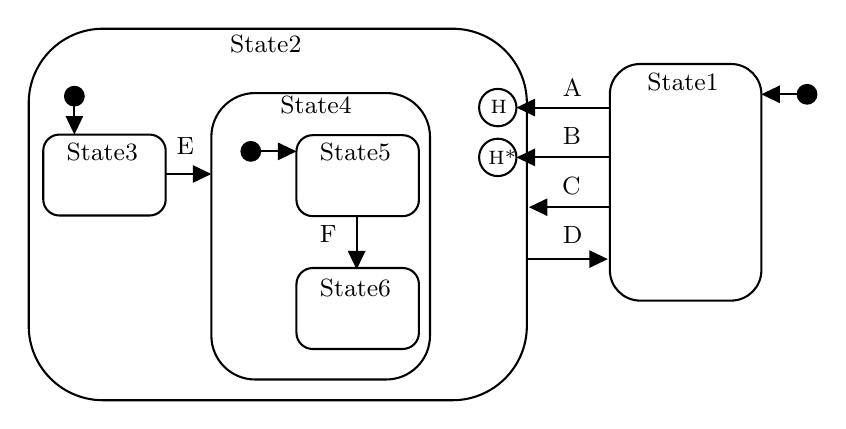
\begin{tikzpicture}[x=0.75pt,y=0.75pt,yscale=-1,xscale=1]
        \draw   (316,91.6) .. controls (316,83.54) and (322.54,77) .. (330.6,77) -- (374.4,77) .. controls (382.46,77) and (389,83.54) .. (389,91.6) -- (389,176.4) .. controls (389,184.46) and (382.46,191) .. (374.4,191) -- (330.6,191) .. controls (322.54,191) and (316,184.46) .. (316,176.4) -- cycle ;
        \draw   (36,95.8) .. controls (36,76.03) and (52.03,60) .. (71.8,60) -- (240.2,60) .. controls (259.97,60) and (276,76.03) .. (276,95.8) -- (276,203.2) .. controls (276,222.97) and (259.97,239) .. (240.2,239) -- (71.8,239) .. controls (52.03,239) and (36,222.97) .. (36,203.2) -- cycle ;
        \draw   (253,98) .. controls (253,93.03) and (257.03,89) .. (262,89) .. controls (266.97,89) and (271,93.03) .. (271,98) .. controls (271,102.97) and (266.97,107) .. (262,107) .. controls (257.03,107) and (253,102.97) .. (253,98) -- cycle ;
        \draw    (316,98) -- (274,98) ;
        \draw [shift={(271,98)}, rotate = 360] [fill={rgb, 255:red, 0; green, 0; blue, 0 }  ][line width=0.08]  [draw opacity=0] (8.93,-4.29) -- (0,0) -- (8.93,4.29) -- cycle    ;
        \draw   (253,122) .. controls (253,117.03) and (257.03,113) .. (262,113) .. controls (266.97,113) and (271,117.03) .. (271,122) .. controls (271,126.97) and (266.97,131) .. (262,131) .. controls (257.03,131) and (253,126.97) .. (253,122) -- cycle ;
        \draw    (316,122) -- (274,122) ;
        \draw [shift={(271,122)}, rotate = 360] [fill={rgb, 255:red, 0; green, 0; blue, 0 }  ][line width=0.08]  [draw opacity=0] (8.93,-4.29) -- (0,0) -- (8.93,4.29) -- cycle    ;
        \draw    (316,146) -- (280,146) ;
        \draw [shift={(277,146)}, rotate = 360] [fill={rgb, 255:red, 0; green, 0; blue, 0 }  ][line width=0.08]  [draw opacity=0] (8.93,-4.29) -- (0,0) -- (8.93,4.29) -- cycle    ;
        %Rounded Rect [id:dp6424365349780641] 
        \draw   (43,118.8) .. controls (43,114.49) and (46.49,111) .. (50.8,111) -- (94.2,111) .. controls (98.51,111) and (102,114.49) .. (102,118.8) -- (102,142.2) .. controls (102,146.51) and (98.51,150) .. (94.2,150) -- (50.8,150) .. controls (46.49,150) and (43,146.51) .. (43,142.2) -- cycle ;
        %Rounded Rect [id:dp8885087551985356] 
        \draw   (124,112.07) .. controls (124,100.43) and (133.43,91) .. (145.07,91) -- (208.27,91) .. controls (219.9,91) and (229.33,100.43) .. (229.33,112.07) -- (229.33,207.93) .. controls (229.33,219.57) and (219.9,229) .. (208.27,229) -- (145.07,229) .. controls (133.43,229) and (124,219.57) .. (124,207.93) -- cycle ;
        %Straight Lines [id:da4708622111725682] 
        \draw    (102,130) -- (121,130) ;
        \draw [shift={(124,130)}, rotate = 180] [fill={rgb, 255:red, 0; green, 0; blue, 0 }  ][line width=0.08]  [draw opacity=0] (8.93,-4.29) -- (0,0) -- (8.93,4.29) -- cycle    ;
        %Rounded Rect [id:dp33519115192592763] 
        \draw   (165,119.1) .. controls (165,114.79) and (168.49,111.3) .. (172.8,111.3) -- (216.2,111.3) .. controls (220.51,111.3) and (224,114.79) .. (224,119.1) -- (224,142.5) .. controls (224,146.81) and (220.51,150.3) .. (216.2,150.3) -- (172.8,150.3) .. controls (168.49,150.3) and (165,146.81) .. (165,142.5) -- cycle ;
        %Rounded Rect [id:dp2464125318153012] 
        \draw   (165,183.1) .. controls (165,178.79) and (168.49,175.3) .. (172.8,175.3) -- (216.2,175.3) .. controls (220.51,175.3) and (224,178.79) .. (224,183.1) -- (224,206.5) .. controls (224,210.81) and (220.51,214.3) .. (216.2,214.3) -- (172.8,214.3) .. controls (168.49,214.3) and (165,210.81) .. (165,206.5) -- cycle ;
        %Straight Lines [id:da18262498013213624] 
        \draw    (194,150) -- (194,173) ;
        \draw [shift={(194,176)}, rotate = 270] [fill={rgb, 255:red, 0; green, 0; blue, 0 }  ][line width=0.08]  [draw opacity=0] (8.93,-4.29) -- (0,0) -- (8.93,4.29) -- cycle    ;
        %Shape: Circle [id:dp7975824864192831] 
        \draw  [fill={rgb, 255:red, 0; green, 0; blue, 0 }  ,fill opacity=1 ] (53.5,92.5) .. controls (53.5,90.01) and (55.51,88) .. (58,88) .. controls (60.49,88) and (62.5,90.01) .. (62.5,92.5) .. controls (62.5,94.99) and (60.49,97) .. (58,97) .. controls (55.51,97) and (53.5,94.99) .. (53.5,92.5) -- cycle ;
        %Shape: Circle [id:dp6700330141668243] 
        \draw  [fill={rgb, 255:red, 0; green, 0; blue, 0 }  ,fill opacity=1 ] (138.5,119.1) .. controls (138.5,116.61) and (140.51,114.6) .. (143,114.6) .. controls (145.49,114.6) and (147.5,116.61) .. (147.5,119.1) .. controls (147.5,121.59) and (145.49,123.6) .. (143,123.6) .. controls (140.51,123.6) and (138.5,121.59) .. (138.5,119.1) -- cycle ;
        %Shape: Circle [id:dp539114832644243] 
        \draw  [fill={rgb, 255:red, 0; green, 0; blue, 0 }  ,fill opacity=1 ] (406.5,91.6) .. controls (406.5,89.11) and (408.51,87.1) .. (411,87.1) .. controls (413.49,87.1) and (415.5,89.11) .. (415.5,91.6) .. controls (415.5,94.09) and (413.49,96.1) .. (411,96.1) .. controls (408.51,96.1) and (406.5,94.09) .. (406.5,91.6) -- cycle ;
        %Straight Lines [id:da3842073346914432] 
        \draw    (392,91.6) -- (411,91.6) ;
        \draw [shift={(389,91.6)}, rotate = 0] [fill={rgb, 255:red, 0; green, 0; blue, 0 }  ][line width=0.08]  [draw opacity=0] (8.93,-4.29) -- (0,0) -- (8.93,4.29) -- cycle    ;
        \draw    (143,119.1) -- (162,119.1) ;
        \draw [shift={(165,119.1)}, rotate = 180] [fill={rgb, 255:red, 0; green, 0; blue, 0 }  ][line width=0.08]  [draw opacity=0] (8.93,-4.29) -- (0,0) -- (8.93,4.29) -- cycle    ;

        \draw    (58,97) -- (58,108) ;
        \draw [shift={(58,111)}, rotate = 270] [fill={rgb, 255:red, 0; green, 0; blue, 0 }  ][line width=0.08]  [draw opacity=0] (8.93,-4.29) -- (0,0) -- (8.93,4.29) -- cycle    ;
        \draw    (312,171) -- (276,171) ;
        \draw [shift={(315,171)}, rotate = 180] [fill={rgb, 255:red, 0; green, 0; blue, 0 }  ][line width=0.08]  [draw opacity=0] (8.93,-4.29) -- (0,0) -- (8.93,4.29) -- cycle    ;
        
        \draw (332.6,80) node [anchor=north west][inner sep=0.75pt]  [font=\small] [align=left] {State1};
        \draw (257,93) node [anchor=north west][inner sep=0.75pt]  [font=\scriptsize] [align=left] {H};
        \draw (256,117) node [anchor=north west][inner sep=0.75pt]  [font=\scriptsize] [align=left] {H*};
        \draw (131.6,62) node [anchor=north west][inner sep=0.75pt]  [font=\small] [align=left] {State2};
        \draw (52.8,114) node [anchor=north west][inner sep=0.75pt]  [font=\small] [align=left] {State3};
        \draw (155.8,91) node [anchor=north west][inner sep=0.75pt]  [font=\small] [align=left] {State4};
        \draw (174.8,114) node [anchor=north west][inner sep=0.75pt]  [font=\small] [align=left] {State5};
        \draw (174.8,179.3) node [anchor=north west][inner sep=0.75pt]  [font=\small] [align=left] {State6};
        \draw (291.8,83) node [anchor=north west][inner sep=0.75pt]  [font=\small] [align=left] {A};
        \draw (291.8,106) node [anchor=north west][inner sep=0.75pt]  [font=\small] [align=left] {B};
        \draw (291.5,130) node [anchor=north west][inner sep=0.75pt]  [font=\small] [align=left] {C};
        \draw (291.8,154) node [anchor=north west][inner sep=0.75pt]  [font=\small] [align=left] {D};
        \draw (105.8,111) node [anchor=north west][inner sep=0.75pt]  [font=\small] [align=left] {E};
        \draw (174.8,153.3) node [anchor=north west][inner sep=0.75pt]  [font=\small] [align=left] {F};
    \end{tikzpicture}

    \caption{Example with history pseudo-states}
    \label{fig:hsmhistory}
\end{figure}

\textit{Shallow history} A transition to the shallow history state in a composite state invokes the last state that was active, at the same depth as the history state itself, prior to the most recent exit of the composite state. 

\textit{Deep history} A transition to the deep history state within a composite state invokes the state that was active, immediately before the most recent exit of the composite state. The last active state can be nested at any depth. 

Here, the way to specify this type of transitions in QuarkTS is very straightforward, you only need to assign the history-mode in the last entry of the transition as shown below:
\medskip

\lstinputlisting[style=CStyle]{historyex1.c}

And here, the configuration and topology of the state-machine is presented, including the default transitions (the small circles filled with black). Please don't forget to define the callbacks for each state.

\medskip
\lstinputlisting[style=CStyle]{historyex2.c}